\documentclass[12pt]{article}

\usepackage[english]{babel}
\usepackage[utf8]{inputenc}
\usepackage{sansmathfonts}
\usepackage[T1]{fontenc}
\renewcommand*\familydefault{\sfdefault} %% Only if the base font of the document is to be sans serif
\usepackage{multicol,lipsum}
\usepackage{amsmath,cancel}
\usepackage{amssymb,amsthm,dsfont,mathrsfs}
\usepackage[colorinlistoftodos]{todonotes}
\usepackage{geometry}
\geometry{
a4paper,
total={170mm,257mm},
left=20mm,
top=15mm,
bottom=22mm,
}
\usepackage{natbib}
\usepackage{soul}
\usepackage{setspace}
\usepackage{hyperref}
\usepackage{xcolor}
\usepackage{graphicx}
\usepackage{tikz}
\usepackage{siunitx}
\graphicspath{ {imagens/} }
\usepackage{fancyhdr}
\pagestyle{fancy}
\renewcommand{\headrulewidth}{0pt}

\color{darkgray}
\newcommand{\T}[1]{\vspace{0.4cm}\textbf{\large#1}}
\newcommand{\TW}[1]{\textbf{\large#1}}

\newcommand{\TM}[1]{\vspace{0.2cm} \textbf{#1}}

\newcommand{\M}[1]{
\vspace{-0.6cm}
\begin{flalign*}
#1&
\end{flalign*}
\vspace{-0.6cm}
}


\definecolor{bluebell}{rgb}{0.25, 0.35, 0.89} 
\definecolor{laranja}{rgb}{0.87, 0.48, 0.25} 
\definecolor{verde}{rgb}{0, 0.54, 0.44} 
\definecolor{babypink}{rgb}{1, 0.42, 0.52} 
\definecolor{rosa}{rgb}{1, 0.72, 0.77} 
\definecolor{cinza}{rgb}{0.3, 0.3, 0.3}  
\definecolor{iris}{rgb}{0.25, 0.35, 0.89}  
\definecolor{babyblue}{rgb}{0.13, 0.59, 0.95}

\setlength\columnsep{30pt}

\setlength{\parindent}{0cm}
\setlength{\fboxrule}{1.3pt}  % <-- Aumenta a espessura

\newcommand{\Formula}[1]{
\begin{center}
\color{iris}
\fcolorbox{rosa}{white}{
\(
\begin{array}{c}
#1
\end{array}
\)
}
\color{cinza}
\end{center}
}

\begin{document}
\pagenumbering{gobble}
\setstretch{1.3}


\includegraphics[width=4cm]{Logo2.png}
\begin{center}
    \textbf{\Huge \textcolor{bluebell}{Semelhança entre Ângulos}}
\end{center}

\begin{multicols}{2}

\TW{Definição} 

Todo ângulo oposto pelo vértice formado por duas semi-retas possuem a mesma medida, ou seja, são ângulos congruentes. Dizemos que dois ângulos são complementares quando a soma entre eles é igual a $\ang{90}$ e suplementar quando a soma é igual a $\ang{180}$.

\begin{center}
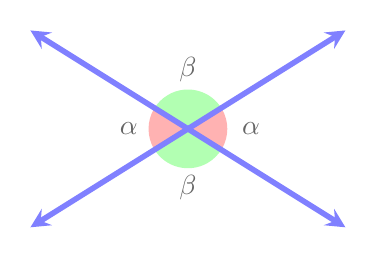
\begin{tikzpicture}
\tikzstyle{texto}=[draw=none,fill=none,black!60!white]
\tikzstyle{line}=[blue!50!white,fill=blue!20!white,line width=2pt]
\tikzstyle{angleA}=[draw=none,fill=red!30!white]
\tikzstyle{angleB}=[draw=none,fill=green!30!white]

\begin{scope}[shift={(2,1.25)}]
    \draw[angleA] (0,0) -- (-30:0.5) arc (-30:30:0.5);
    \draw[angleA] (0,0) -- (150:0.5) arc (150:210:0.5);
    \draw[angleB] (0,0) -- (30:0.5) arc (30:150:0.5);
    \draw[angleB] (0,0) -- (210:0.5) arc (210:330:0.5);
\end{scope}

\draw[line,stealth-stealth] (0,0) -- (4,2.5);
\draw[line,stealth-stealth] (0,2.5) -- (4,0);
\node[texto] at (1.25,1.25) {\textbf{$\alpha$}};
\node[texto] at (2.8,1.25) {\textbf{$\alpha$}};
\node[texto] at (2,2) {\textbf{$\beta$}};
\node[texto] at (2,0.5) {\textbf{$\beta$}};
\end{tikzpicture}
\end{center}

\TM{Exemplo:}

\begin{center}
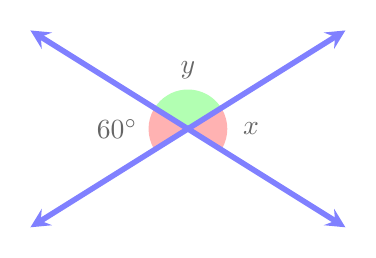
\begin{tikzpicture}
\tikzstyle{texto}=[draw=none,fill=none,black!60!white]
\tikzstyle{line}=[blue!50!white,fill=blue!20!white,line width=2pt]
\tikzstyle{angleA}=[draw=none,fill=red!30!white]
\tikzstyle{angleB}=[draw=none,fill=green!30!white]

\begin{scope}[shift={(2,1.25)}]
    \draw[angleA] (0,0) -- (-30:0.5) arc (-30:30:0.5);
    \draw[angleA] (0,0) -- (150:0.5) arc (150:210:0.5);
    \draw[angleB] (0,0) -- (30:0.5) arc (30:150:0.5);
\end{scope}

\draw[line,stealth-stealth] (0,0) -- (4,2.5);
\draw[line,stealth-stealth] (0,2.5) -- (4,0);
\node[texto] at (1.1,1.25) {\textbf{$\ang{60}$}};
\node[texto] at (2.8,1.25) {\textbf{$x$}};
\node[texto] at (2,2) {\textbf{$y$}};
\end{tikzpicture}
\end{center}

Conforme definição deduzimos que $x=\ang{60}$. Como $y$ é suplemento de $x$ então temos que:

$y + x = 180$

$y = 180 - x$

$y = 180 - 60$

$y = 120$


\T{Retas paralelas}

Os ângulos correspondentes formados por duas retas paralelas e uma transversal são iguais (congruentes). Na figura abaixo temos duas retas paralelas $s$ e $r$ que são cortadas por uma reta transversal formando 4 ângulos $\alpha$ e 4 ângulos $\beta$ de modo que $\alpha$ é suplemento de $\beta$.

\begin{center}
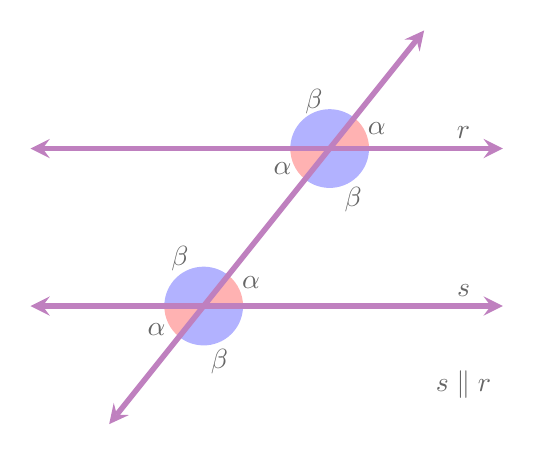
\begin{tikzpicture}
\tikzstyle{texto}=[draw=none,fill=none,black!60!white]
\tikzstyle{line}=[violet!50!white,line width=2pt]
\tikzstyle{angleA}=[draw=none,fill=red!30!white]
\tikzstyle{angleB}=[draw=none,fill=blue!30!white]
\begin{scope}[shift={(3.8,2)}]
    \draw[angleA] (0,0) -- (0:0.5) arc (0:50:0.5);
    \draw[angleA] (0,0) -- (180:0.5) arc (180:230:0.5);
    \draw[angleB] (0,0) -- (50:0.5) arc (50:180:0.5);
    \draw[angleB] (0,0) -- (230:0.5) arc (230:360:0.5);
\end{scope}

\begin{scope}[shift={(2.2,0)}]
    \draw[angleA] (0,0) -- (0:0.5) arc (0:50:0.5);
    \draw[angleA] (0,0) -- (180:0.5) arc (180:230:0.5);
    \draw[angleB] (0,0) -- (50:0.5) arc (50:180:0.5);
    \draw[angleB] (0,0) -- (230:0.5) arc (230:360:0.5);
\end{scope}

\draw[line,stealth-stealth] (0,0) -- (6,0);
\draw[line,stealth-stealth] (0,2) -- (6,2);
\draw[line,stealth-stealth] (1,-1.5) -- (5,3.5);

\node[texto] at (4.4,2.25) {\textbf{$\alpha$}};
\node[texto] at (3.2,1.75) {\textbf{$\alpha$}};
\node[texto] at (2.8,0.3) {\textbf{$\alpha$}};
\node[texto] at (1.6,-0.3) {\textbf{$\alpha$}};
\node[texto] at (3.6,2.6) {\textbf{$\beta$}};
\node[texto] at (4.1,1.35) {\textbf{$\beta$}};
\node[texto] at (1.9,0.6) {\textbf{$\beta$}};
\node[texto] at (2.4,-0.7) {\textbf{$\beta$}};

\node[texto] at (5.5,0.2) {\textbf{$s$}};
\node[texto] at (5.5,2.2) {\textbf{$r$}};
\node[texto] at (5.5,-1) {\textbf{$s \parallel r$}};
\end{tikzpicture}
\end{center}

\TM{Exemplo:}

\begin{center}
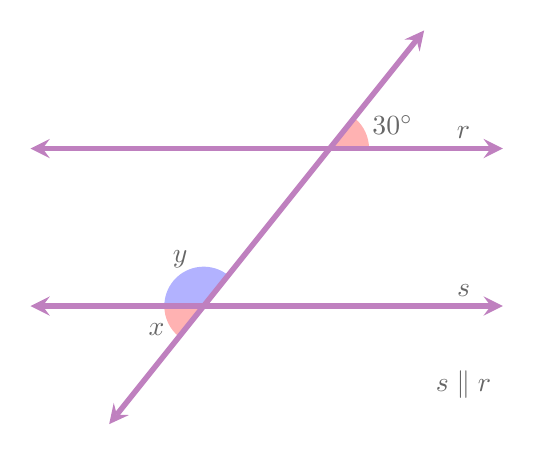
\begin{tikzpicture}
\tikzstyle{texto}=[draw=none,fill=none,black!60!white]
\tikzstyle{line}=[violet!50!white,line width=2pt]
\tikzstyle{angleA}=[draw=none,fill=red!30!white]
\tikzstyle{angleB}=[draw=none,fill=blue!30!white]
\begin{scope}[shift={(3.8,2)}]
    \draw[angleA] (0,0) -- (0:0.5) arc (0:50:0.5);
    %\draw[angleA] (0,0) -- (180:0.5) arc (180:230:0.5);
    %\draw[angleB] (0,0) -- (50:0.5) arc (50:180:0.5);
    %\draw[angleB] (0,0) -- (230:0.5) arc (230:360:0.5);
\end{scope}

\begin{scope}[shift={(2.2,0)}]
   % \draw[angleA] (0,0) -- (0:0.5) arc (0:50:0.5);
    \draw[angleA] (0,0) -- (180:0.5) arc (180:230:0.5);
    \draw[angleB] (0,0) -- (50:0.5) arc (50:180:0.5);
    %\draw[angleB] (0,0) -- (230:0.5) arc (230:360:0.5);
\end{scope}

\draw[line,stealth-stealth] (0,0) -- (6,0);
\draw[line,stealth-stealth] (0,2) -- (6,2);
\draw[line,stealth-stealth] (1,-1.5) -- (5,3.5);

\node[texto] at (4.6,2.3) {\textbf{$\ang{30}$}};
%\node[texto] at (3.2,1.75) {\textbf{$\alpha$}};
%\node[texto] at (2.8,0.3) {\textbf{$\alpha$}};
\node[texto] at (1.6,-0.3) {\textbf{$x$}};
%\node[texto] at (3.6,2.6) {\textbf{$\beta$}};
%\node[texto] at (4.1,1.35) {\textbf{$\beta$}};
\node[texto] at (1.9,0.6) {\textbf{$y$}};
%\node[texto] at (2.4,-0.7) {\textbf{$\beta$}};

\node[texto] at (5.5,0.2) {\textbf{$s$}};
\node[texto] at (5.5,2.2) {\textbf{$r$}};
\node[texto] at (5.5,-1) {\textbf{$s \parallel r$}};
\end{tikzpicture}
\end{center}

Neste exemplo temos que $x=\ang{30}$ e $y + x = 180 $.

$y + 30 = 180 $


$y = 180 - 30 $

$y = 150$

\end{multicols}

\lfoot{\scriptsize © Copyright, Pratique Já}
\cfoot{\large \textcolor{bluebell}{pratiqueja.com}}
\end{document}